\section{Methodological Detail - Text Embeddings}

Text embeddings were computed for each post by inputting the post text into \mbox{OpenAI's} \texttt{text-embedding-3-small} embedding model. The embedding model computes a 1,536 dimensional embedding vector for each post that encodes the meaning of the text in such a way that two posts with similar text will have a small distance between their embedding vectors. The raw embedding dimensions are learned from a large general purpose training corpus and are not tailored to the structure of our dataset. We therefore compute the principal components of the raw embedding vectors using our corpus. The principal components are orthogonal linear combinations of the original 1,536 embedding dimensions that explain the greatest variation across posts in our data. Figure \ref{fig_text_scree_plot} shows the scree plot of the principal components analysis, for the first \gn{NumPCAComponentsShow} components. To keep our regression in \eqref{eq_zreg} parsimonious, we decided to use only the first \gn{TextPCAK} components in the analysis. These components explain  \gn{TextPCAPctExplained}\% of the total variation,  but our results in Section \ref{sec_v4v} are robust to the specific choice of how many components to use. After running regression \eqref{eq_zreg}, we inspected the embedding dimensions that were most predictive of zaps. The first most predictive dimension appears to capture meta-posts (not necessarily in the \texttt{meta} territory) about Stacker News itself, such as tips for how to post and earn more sats. The second most predictive dimension appears to capture posts about geopolitical and macroeconomic events, such as a personal discussion about elections in Venezuela. The third most predictive dimension appears to capture posts that ask questions about personal finance. We note that, although these embedding dimensions are the most strongly associated with zaps, other predictive aspects of the text content may not align with any single dimension and may instead be captured by combinations of dimensions. We therefore treat the embedding components primarily as control variables in the regression and avoid over-interpreting individual coefficients or assigning strong substantive meaning to any single dimension.

\pagebreak

\begin{figure}[H]
\caption{Scree Plot for Post Text Embeddings}
\label{fig_text_scree_plot}
\vspace{-0.6cm}
\begin{center}
\begin{adjustbox}{width=\textwidth}
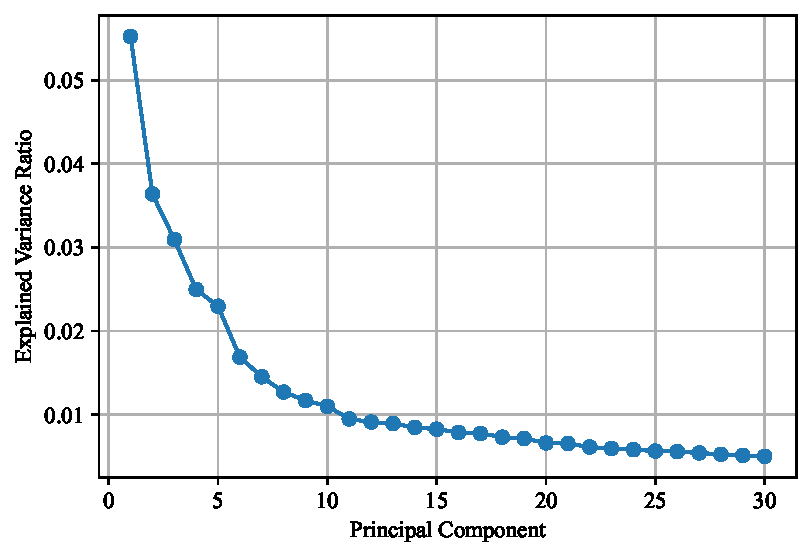
\includegraphics{results/fig_text_scree_plot.pdf}
\end{adjustbox}
\end{center}
\footnotesize \textit{Note:} Shows the scree plot for post text embeddings, indicating the explained variance ratio for each principal component. 
The total explained variance at $K=10$ is \gn{TextPCAPctExplained}\%.
\end{figure}

